\documentclass{beamer}

\usepackage{import}
\usepackage{xifthen}
\usepackage{pdfpages}
\usepackage{transparent}



% This file is a solution template for:

% - Talk at a conference/colloquium.
% - Talk length is about 20min.
% - Style is ornate.



% Copyright 2004 by Till Tantau <tantau@users.sourceforge.net>.
%
% In principle, this file can be redistributed and/or modified under
% the terms of the GNU Public License, version 2.
%
% However, this file is supposed to be a template to be modified
% for your own needs. For this reason, if you use this file as a
% template and not specifically distribute it as part of a another
% package/program, I grant the extra permission to freely copy and
% modify this file as you see fit and even to delete this copyright
% notice. 


\mode<presentation>
{
  \usetheme{Berlin}
  \setbeamercovered{transparent}
  \setbeamertemplate{caption}[numbered]
}


\usepackage[spanish,mexico]{babel}
% \usepackage[utf8]{inputenc}
\usepackage{times}
\usepackage[T1]{fontenc}

\title{Péndulo Simple}

\subtitle
{Modelado, simulación y resultados}

\author[Benavides Et Al.]{E. Benavides \and I. Ayala \and S. Campos \\ \and L. Almazán \and Y. Casas}


\institute[]
{
  Centro de Investigación y de Estudios Avanzados del IPN\\
  Robótica y Manufactura Avanzada
  }

\date[]{RyMA 2019}

\subject{System Modeling}



% Delete this, if you do not want the table of contents to pop up at
% the beginning of each subsection:
\AtBeginSubsection[]
{
  \begin{frame}<beamer>{Outline}
    \tableofcontents[currentsection,currentsubsection]
  \end{frame}
}


% If you wish to uncover everything in a step-wise fashion, uncomment
% the following command: 

%\beamerdefaultoverlayspecification{<+->}



\begin{document}




\begin{frame}
  \titlepage
\end{frame}

\begin{frame}{Contenido}
  \tableofcontents
\end{frame}



\section{Introducción}

\subsection{Nomenclatura}
\begin{frame}{Definiciones}
\begin{itemize}
 \item 
\end{itemize}

 
\end{frame}


\subsection{Objetivos}

\begin{frame}{Objetivos del proyecto}

  \begin{itemize}
    \item 
  \end{itemize}
  
\end{frame}

\section{Modelo matemático}

\subsection{Cinemática}

\begin{frame}{Diagrama del péndulo}
 \begin{figure}[ht]
    \centering
    \import{../Report/img/}{pendulum_diagram.pdf_tex}
    \caption{Sistema de Péndulo simple.}
    \label{fig: simple pendulum}
\end{figure}

\end{frame}

\begin{frame}{Método de Newton}

\begin{itemize}
 \item 
 \begin{equation}
  \sum F = -F_{mg} - F_f 
 \end{equation}

\end{itemize}

\end{frame}

\begin{frame}{Método de Newton}
\begin{itemize}
 \item 
\end{itemize}
\end{frame}

\begin{frame}{Método de conservación de energía}
 \begin{itemize}
  \item   
 \end{itemize}
\end{frame}


\begin{frame}{Método de conservación de energía}
\begin{itemize}
 \item
\end{itemize}
\end{frame}


\section{Simulación}
\subsection{Software}
\begin{frame}{MATLAB}
 \begin{itemize}
  \item Se simularon las ecuaciones de movimiento del sistema con las siguientes condiciones de simulación.
 \end{itemize}

\end{frame}


\subsection{Resultados}

\begin{frame}{Modelo matemático}
 \begin{figure}[h]
 \centering
 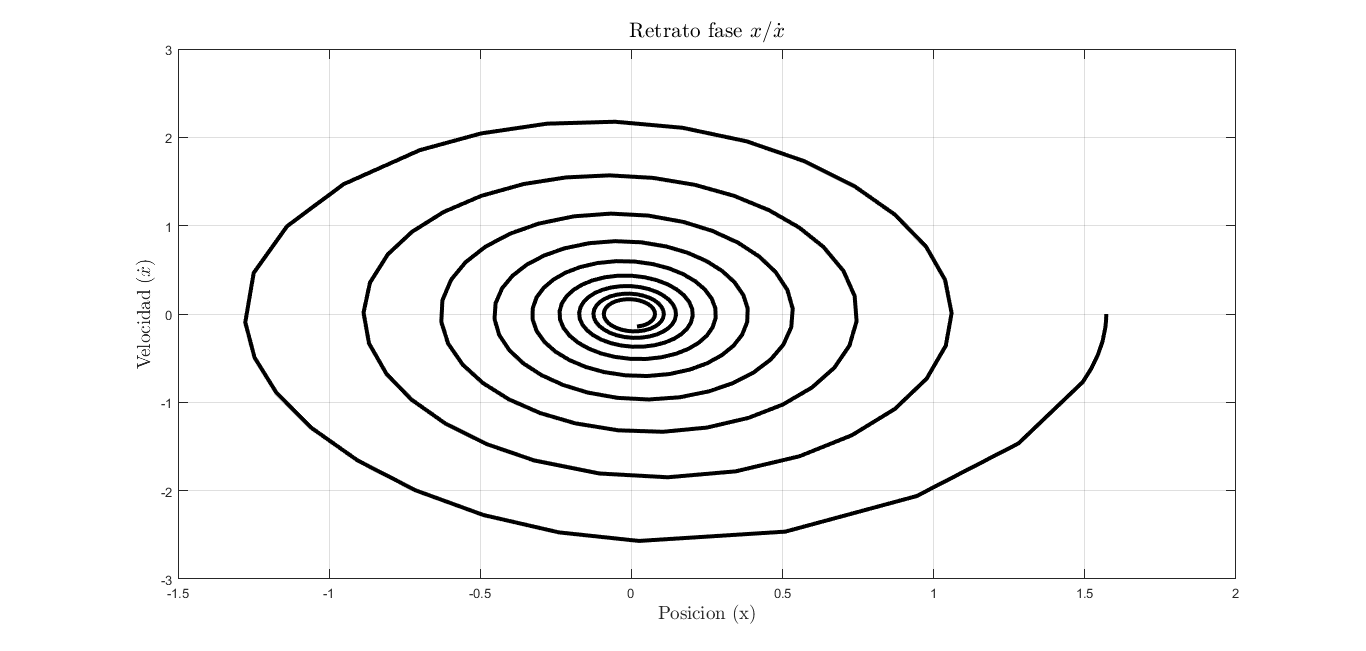
\includegraphics[scale=0.2]{../Report/img/fasependulox2.png}
 % fasependulox2.png: 1366x651 px, 96dpi, 36.14x17.22 cm, bb=0 0 1024 488
 \caption{Diagrama de fase de $x$ y $\dot{x}$ del modelo matemático.}
 \label{fig: matlab phase diagram x vx}
\end{figure}

\end{frame}

\begin{frame}{Modelo matemático}
  \begin{figure}[h]
 \centering
 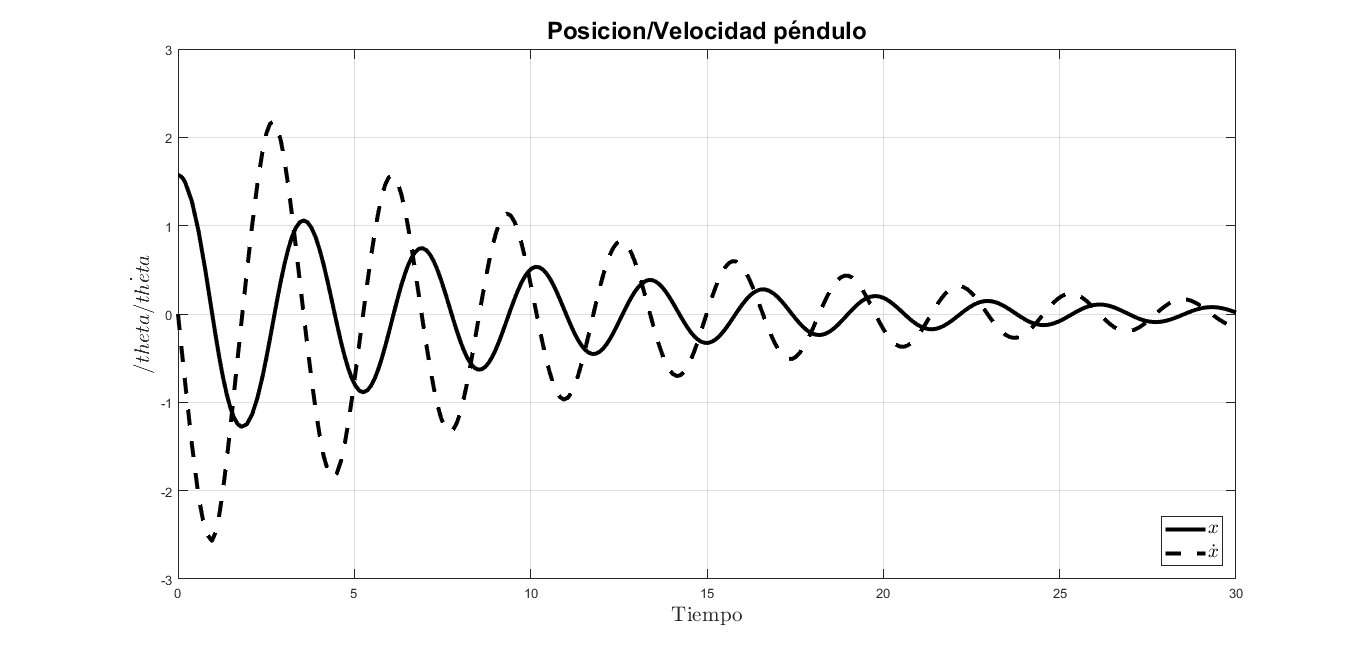
\includegraphics[scale=0.2]{../Report/img/posvelpendulo2.png}
 % fasependulox2.png: 1366x651 px, 96dpi, 36.14x17.22 cm, bb=0 0 1024 488
 \caption{Gráfica respecto al tiempo de $\theta$ y $\dot{\theta}$ del modelo matemático.}
 \label{fig: matlab plot x vx}
\end{figure}

\end{frame}


\section{Modelo físico}

\subsection{Prueba de concepto}
\begin{frame}{LEGO Mindstorm}
%  TODO Insert image of the Mindstorm pendulum here

\end{frame}

\begin{frame}{Análisis de movimiento}
 \begin{figure}[h]
 \centering
 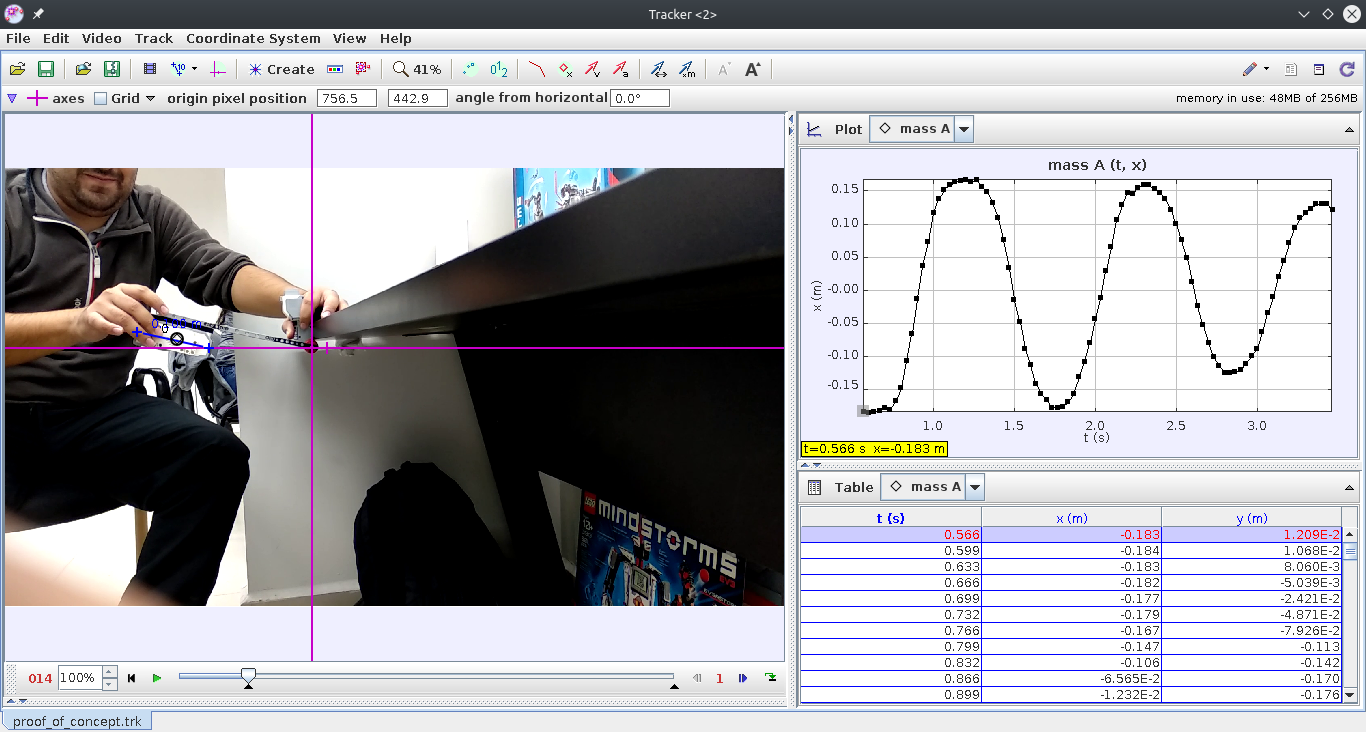
\includegraphics[scale=0.2]{../Report/img/tracker_poc.png}
 % tracker_poc.png: 1366x732 px, 96dpi, 36.14x19.37 cm, bb=0 0 1024 549
 \caption{Análisis de movimiento - Prueba de concepto.}
 \label{fig: tracker main window}
\end{figure}

\end{frame}

\subsection{Resultados}
\begin{frame}{Modelo Físico}
 \begin{figure}[h]
 \centering
 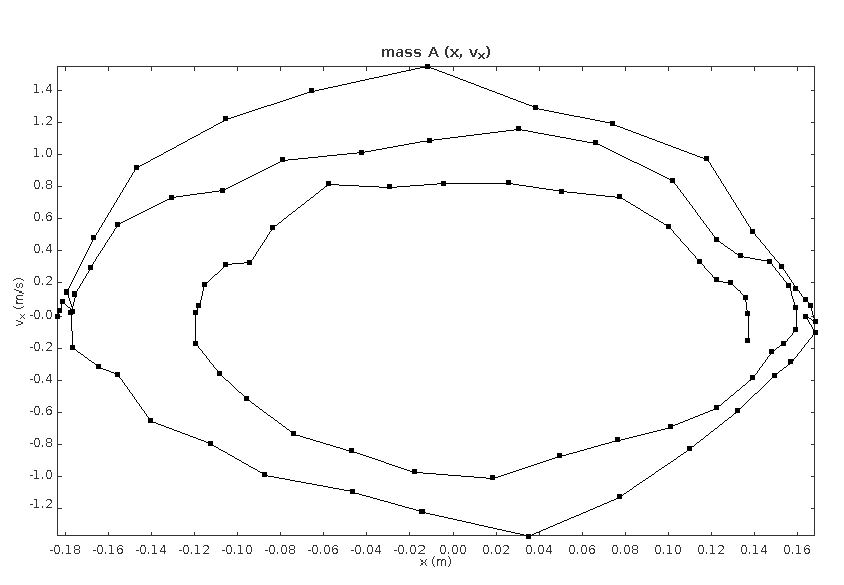
\includegraphics[scale=0.2]{../Report/img/tracker_poc_phasediagram_x_vx.png}
 % tracker_poc_phasediagram_x_vx.png: 844x585 px, 72dpi, 29.78x20.64 cm, bb=0 0 844 585
 \caption{Diagrama de fase de $x$ y $\dot{x}$ del modelo físico.}
 \label{fig: tracker phase diagram x vx}
\end{figure}

\end{frame}

\begin{frame}{Modelo Físico}
 \begin{figure}[h]
 \centering
 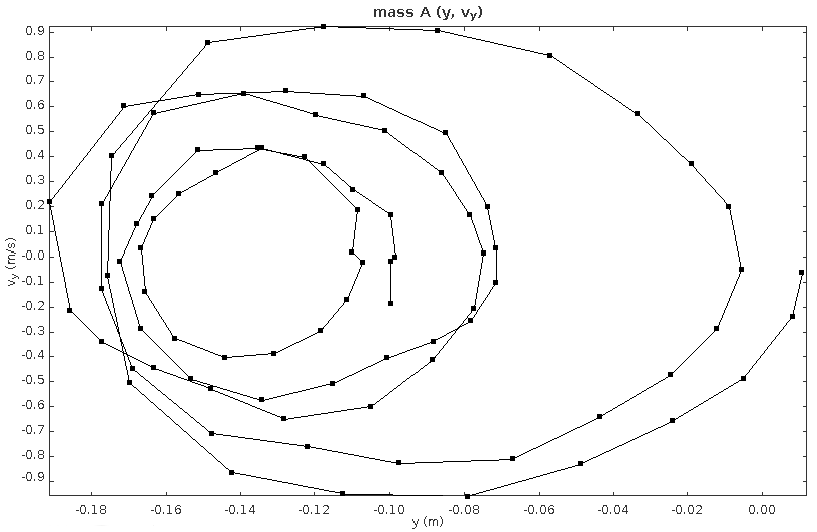
\includegraphics[scale=0.2]{../Report/img/tracker_poc_phasediagram_y_vy.png}
 % tracker_poc_phasediagram_x_vx.png: 844x585 px, 72dpi, 29.78x20.64 cm, bb=0 0 844 585
 \caption{Diagrama de fase de $y$ y $\dot{y}$ del modelo físico.}
 \label{fig: tracker phase diagram y vy}
\end{figure}

\end{frame}

\end{document}


